
%%%%%%%%%%%%%%%%%%%%%%%%%%%%%%%%%%%%%%%%%%%%%%%%%%%%%%%%%%%%%%%%%%%%%%%
%%%%%%%%%%%%%%%%%%%%%%%%%%%%%%%%%%%%%%%%%%%%%%%%%%%%%%%%%%%%%%%%%%%%%%%
%%%%%%%%%%%%%%%%%%%%%%%%%%%%%%%%%%%%%%%%%%%%%%%%%%%%%%%%%%%%%%%%%%%%%%%

\begin{frame}{The Neyman-Scott ``paradox''}
\begin{figure}
    \centering
    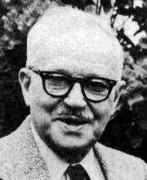
\includegraphics[height=0.2\textwidth]{static_images/neyman.jpg}
    
\includegraphics[height=0.2\textwidth]{static_images/ElizabethScott.jpg}
\end{figure}

...or why don't we always use the maximum likelihood estimator?

\hrulefill

Here's a toy model.  For some unknown $z_n$ and $\theta$, draw

\begin{align*}
    y_{na} | z_n, \theta \sim{}& \mathcal{N}(z_n, \theta)\\
    y_{nb} | z_n, \theta \sim{}& \mathcal{N}(z_n, \theta)
\end{align*}


\begin{align*}
    \textrm{Observations: }y ={}& (y_{11}, y_{1b}, \ldots, y_{Na}, y_{Nb})\\
    \textrm{Unknown latent variables: }z ={}& (z_1, \ldots, y_N)\\
    \textrm{Unknown global parameter: }\theta \in \mathbb{R}
\end{align*}

Task: infer $\theta$.

\end{frame}


%%%%%%%%%%%%%%%%%%%%%%%%%%%%%%%%%%%%%%%%%%%%%%%%%%%%%%%%%%%%%%%%%%%%%%%
%%%%%%%%%%%%%%%%%%%%%%%%%%%%%%%%%%%%%%%%%%%%%%%%%%%%%%%%%%%%%%%%%%%%%%%
%%%%%%%%%%%%%%%%%%%%%%%%%%%%%%%%%%%%%%%%%%%%%%%%%%%%%%%%%%%%%%%%%%%%%%%

\begin{frame}{The Neyman-Scott ``paradox''}

\begin{align*}
    y_{na} | z_n, \theta \sim{} \mathcal{N}(z_n, \theta) \quad\quad\quad
    y_{nb} | z_n, \theta \sim{} \mathcal{N}(z_n, \theta)
\end{align*}

Let's use that old workhorse, the maximum likelihood estimator (MLE)!

(\textbf{Spoiler:} Something will go wrong.)

The normal distribution gives (up to constants):

%
\begin{align*}
%
\log p(y_{na}, y_{nb} | \theta, z_n) ={}&
-\frac{1}{2} \theta^{-1} \left( y_{na}  - z_n\right)^2 - \frac{1}{2}log \theta
&-\frac{1}{2} \theta^{-1} \left( y_{nb}  - z_n\right)^2 - \frac{1}{2}\log \theta
%
\end{align*}
%

\begin{align*}
%
\log p(y | \theta, z) ={}&
\sum_{n=1}^N \log p(y_{na}, y_{nb} | \theta, z_n)
%
\end{align*}
%

The MLE is given by:

%
\begin{align*}
%
\hat\theta, \hat{z} :={}& \argmax_{\theta, z}  \log p(y | \theta, z)
\quad\quad\Leftrightarrow{}\quad\quad
\fracat{\partial \log p(y | \theta, z)}{\partial (\theta, z)}{\thetahat, \hat{z}} ={} 0
%
\end{align*}
%

\textbf{Exercise:} Find an expression for $\hat{z}_n$.

\end{frame}




%%%%%%%%%%%%%%%%%%%%%%%%%%%%%%%%%%%%%%%%%%%%%%%%%%%%%%%%%%%%%%%%%%%%%%%
%%%%%%%%%%%%%%%%%%%%%%%%%%%%%%%%%%%%%%%%%%%%%%%%%%%%%%%%%%%%%%%%%%%%%%%
%%%%%%%%%%%%%%%%%%%%%%%%%%%%%%%%%%%%%%%%%%%%%%%%%%%%%%%%%%%%%%%%%%%%%%%

\begin{frame}{The Neyman-Scott ``paradox''}

\textbf{Exercise:} Find an expression for $\hat{z}_n$.

\begin{align*}
%
0 ={}& \fracat{\partial \log p(y | \theta, z)}{\partial z_n}{\hat{z}, \thetahat} \\
={}& \fracat{\partial \log p(y_{na}, y_{nb} | \theta, z_n)}{\partial z_n}{\hat{z}, \thetahat}\\
={}& \frac{\partial}{\partial z_n}
\left(
-\frac{1}{2} \theta^{-1} \left( y_{na}  - z_n\right)^2 - \frac{1}{2}\log \theta
-\frac{1}{2} \theta^{-1} \left( y_{nb}  - z_n\right)^2 - \frac{1}{2}\log \theta
\right)
\Bigg|_{\hat{z}, \thetahat}\\
={}& - \thetahat^{-1} (y_{na}  - \hat{z}_n)
    - \thetahat^{-1} (y_{nb}  - \hat{z}_n) \Rightarrow \\
\hat{z}_n ={}& \frac{1}{2}(y_{na} + y_{nb}).
%
\end{align*}

Wonderful!  This is a very sensible expression, and it doesn't depend on
$\thetahat$.

\vspace{1em}
\textbf{Exercise:} Using this result, find an expression for $\thetahat$.

Hint:
%
$
%
\left( y_{na}  - \hat{z}_n\right)^2 =
\left( y_{nb}  - \hat{z}_n\right)^2 =
\frac{1}{4} \left( y_{na}  - y_{nb}\right)^2
%
$
%

\end{frame}



%%%%%%%%%%%%%%%%%%%%%%%%%%%%%%%%%%%%%%%%%%%%%%%%%%%%%%%%%%%%%%%%%%%%%%%
%%%%%%%%%%%%%%%%%%%%%%%%%%%%%%%%%%%%%%%%%%%%%%%%%%%%%%%%%%%%%%%%%%%%%%%
%%%%%%%%%%%%%%%%%%%%%%%%%%%%%%%%%%%%%%%%%%%%%%%%%%%%%%%%%%%%%%%%%%%%%%%

\begin{frame}{The Neyman-Scott ``paradox''}

\textbf{Exercise:} Find an expression for $\thetahat$.

Hint:
%
$%
\left( y_{na}  - \hat{z}_n\right)^2 =
\left( y_{nb}  - \hat{z}_n\right)^2 =
\frac{1}{4} \left( y_{na}  - y_{nb}\right)^2
%
$
%

\begin{align*}
%
0 ={}& \fracat{\partial \log p(y | \theta, z)}{\partial \theta}{\hat{z}, \thetahat} \\
={}& \frac{\partial}{\partial \theta}
\sumn
\left(
-\frac{1}{2} \theta^{-1} \left( y_{na}  - z_n\right)^2 - \frac{1}{2}\log \theta
-\frac{1}{2} \theta^{-1} \left( y_{nb}  - z_n\right)^2 - \frac{1}{2}\log \theta
\right)
\Bigg|_{\hat{z}, \thetahat}\\
={}&
\sumn
\left(
\frac{1}{2} \thetahat^{-2} \frac{1}{4} \left( y_{na}  - y_{nb}\right)^2 - \frac{1}{2}\thetahat^{-1} +
\frac{1}{2} \thetahat^{-2} \frac{1}{4} \left( y_{na}  - y_{nb}\right)^2 - \frac{1}{2}\thetahat^{-1}
\right)
\\={}&
\thetahat^{-2} \frac{1}{4} \sumn \left( y_{na}  - y_{nb}\right)^2 - N \thetahat^{-1}
\Rightarrow \\
\thetahat ={}& \frac{1}{4} \meann \left( y_{na}  - y_{nb}\right)^2.
%
\end{align*}

\textbf{Exercise:}
Suppose the true parameters are $\theta_0$ and $z_0$.

What is the behavior of $\thetahat$ for large $N$?

Hint: Use the law of large numbers.

\end{frame}



%%%%%%%%%%%%%%%%%%%%%%%%%%%%%%%%%%%%%%%%%%%%%%%%%%%%%%%%%%%%%%%%%%%%%%%
%%%%%%%%%%%%%%%%%%%%%%%%%%%%%%%%%%%%%%%%%%%%%%%%%%%%%%%%%%%%%%%%%%%%%%%
%%%%%%%%%%%%%%%%%%%%%%%%%%%%%%%%%%%%%%%%%%%%%%%%%%%%%%%%%%%%%%%%%%%%%%%

\begin{frame}{The Neyman-Scott ``paradox''}

\textbf{Exercise:}
What is the behavior of $\thetahat$ for large $N$?
By the law of large numbers,
%
\begin{columns}
%
\begin{column}{0.7\textwidth}
\begin{align*}
%
\thetahat &={} \frac{1}{4} \meann \left( y_{na}  - y_{nb}\right)^2\\
&\plim{} \frac{1}{4}
\expect{p(y | \theta_0, z_0)}{\left( y_{na}  - y_{nb}\right)^2}
\\&=
\frac{1}{4}
\expect{p(y | \theta_0, z_0)}{\left( y_{na} - z_{0n} - (y_{nb} - z_{0n})\right)^2}
\\&=
\frac{1}{4}\Bigg(
    \expect{p(y | \theta_0, z_0)}{( y_{na} - z_{0n})^2} +
    \expect{p(y | \theta_0, z_0)}{( y_{nb} - z_{0n})^2} +
    \\&\quad\quad\quad\quad
    2 \expect{p(y | \theta_0, z_0)}{( y_{na} - z_{0n})( y_{nb} - z_{0n})}
\Bigg)
\\&=
\frac{1}{4}\left(\theta_0 + \theta_0 + 0\right)
\\&= \frac{\theta_0}{2} \ne \theta_0.
%
\end{align*}
%
\end{column}
\begin{column}{0.3\textwidth}
    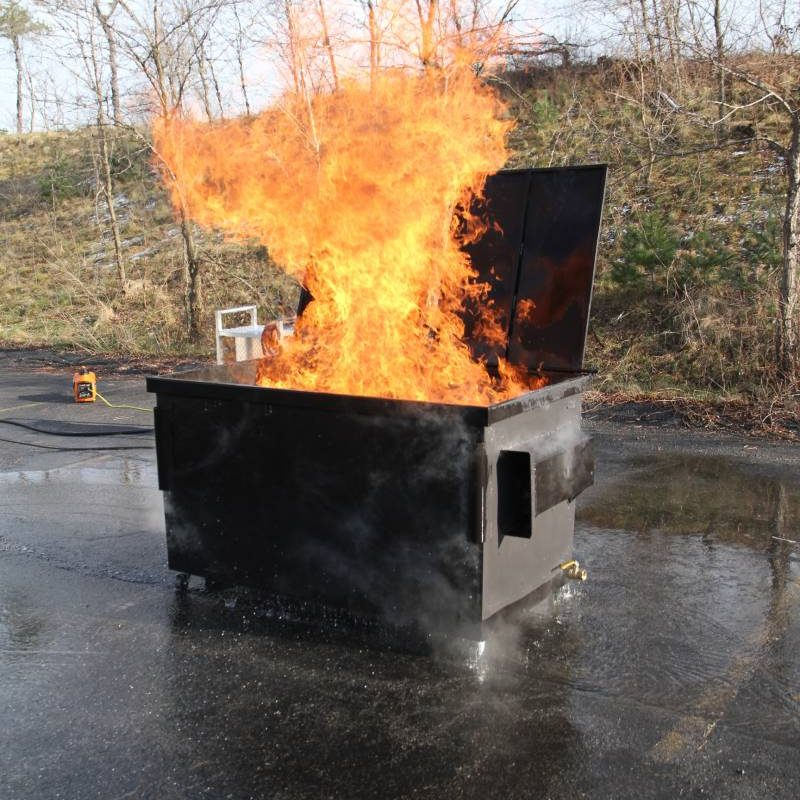
\includegraphics[width=1.0\textwidth]{static_images/dumpster.jpg}
\end{column}
\end{columns}

\vspace{2em}
$\Rightarrow$ \textbf{The MLE is inconsistent.  What went wrong?}

\end{frame}


%%%%%%%%%%%%%%%%%%%%%%%%%%%%%%%%%%%%%%%%%%%%%%%%%%%%%%%%%%%%%%%%%%%%%%%
%%%%%%%%%%%%%%%%%%%%%%%%%%%%%%%%%%%%%%%%%%%%%%%%%%%%%%%%%%%%%%%%%%%%%%%
%%%%%%%%%%%%%%%%%%%%%%%%%%%%%%%%%%%%%%%%%%%%%%%%%%%%%%%%%%%%%%%%%%%%%%%

\begin{frame}{The Neyman-Scott ``paradox''}

\textbf{The MLE is inconsistent.  What went wrong?}

\begin{align*}
\hat{z_n} &= \frac{1}{2}(y_{na} + y_{nb}) \\
\thetahat &\plim \frac{\theta_0}{2} \ne \theta_0
\end{align*}

\begin{columns}
    \begin{column}{0.8\textwidth}
\begin{itemize}
    %
\item Our estimates for the latent variables $\hat{z}_n$ are quite uncertain (they use only
two observaitons each)
%
\item But our MLE estimate for $\thetahat$ treated the $\hat{z}_n$ as if they
were known exactly
%
\item $\Rightarrow$ We estimated less dispersion around $\hat{z}_n$ than was
truly present.  That is, we \emph{under-estimated} the dispersion $\theta_0$.
%
\item To avoid this problem, we must \emph{account for the uncertainty} in $\z_n$
when estimating $\theta$.
%
\end{itemize}
\end{column}
\end{columns}

\vspace{2em}
Solution: \textbf{Marginalization.}

\end{frame}




%%%%%%%%%%%%%%%%%%%%%%%%%%%%%%%%%%%%%%%%%%%%%%%%%%%%%%%%%%%%%%%%%%%%%%%
%%%%%%%%%%%%%%%%%%%%%%%%%%%%%%%%%%%%%%%%%%%%%%%%%%%%%%%%%%%%%%%%%%%%%%%
%%%%%%%%%%%%%%%%%%%%%%%%%%%%%%%%%%%%%%%%%%%%%%%%%%%%%%%%%%%%%%%%%%%%%%%

\begin{frame}{The Neyman-Scott ``paradox''}

To marginalize we must:

\begin{itemize}
\item Add a distributional assumption $z | \theta \sim p(z \vert \theta)$.
\item Compute the marginal $p(y | \theta) = \int p(y | \theta, z) p(z \vert \theta) d z$.
\item Compute the marginal MLE $\thetahat = \argmax{\theta} p(y | \theta)$
\begin{itemize}
    \item (Contrast with $\thetahat, \hat{z} = \argmax_{\theta, z} p(y | \theta, z)$)
\end{itemize}
\end{itemize}

%$p(y_{na}, y_{nb} | \theta) = \int p(y_{na}, y_{nb} | \theta, z_n) p(z_n) d z_n$.

\textbf{Neyman-Scott resolved}

Let's let $z_n \sim \mathcal{N}(0, 1)$.  Then, by standard properties of the
normal,
%
\begin{align*}
%
\left(
\begin{array}{c}
    y_{na} \\
    y_{nb}
\end{array}
\right)
\iid
\mathcal{N}\left(
\left(
\begin{array}{c}
    0 \\
    0
\end{array}
\right),
%
\left(
\begin{array}{cc}
    1 + \theta& 1 \\
    1& 1 + \theta \\
\end{array}
\right)
%
\right)
%
\end{align*}
%
Sample covariances of the bivariate normal are consistent, so
%
\begin{align*}
%
\thetahat := \argmax_\theta \sumn \log \int p(y_{na}, y_{nb} | \theta, z_n) p(z_n) dz_n
%
\end{align*}
%
is consistent.





\end{frame}
